\documentclass{appolb}
\usepackage{graphicx}
\usepackage{multirow}
\usepackage{tabularx} 
\usepackage{rotating,graphicx} 
\usepackage{appendix} 
\usepackage{makecell}
\usepackage{amsmath}
\usepackage{amssymb}
\usepackage{cite}
\usepackage[T1]{fontenc}
\usepackage{amsmath}
\usepackage[amssymb]{SIunits}
\usepackage{hyperref}

\usepackage{lineno}
\linenumbers

% graphicx package included for placing figures in the text
%------------------------------------------------------
% $Id: commands.tex 909 2013-06-03 14:10:59Z rpreghen $
% Adaptation of a file originally by Roberto Preghenella (thanks!) 
%==========================================================%
\newcommand{\btwo}{\ensuremath{B_{2}}}
\newcommand{\bthree}{\ensuremath{B_{3}}}
\newcommand{\bA}{\ensuremath{B_{A}}}
\newcommand{\bthreeLambda}{$B_{3, \Lambda}$}

%nuclei and hypernuclei
\newcommand{\tritium}{\ensuremath{{}^{3}\mathrm{H}}}
\newcommand{\hethree}{\ensuremath{{}^{3}\mathrm{He}}}
\newcommand{\hefour}{\ensuremath{{}^{4}\mathrm{He}}}
\newcommand{\hthreelambda}{\ensuremath{{}^{3}_{\Lambda}\mathrm{H}}}
\newcommand{\hfourlambda}{\ensuremath{{}^{4}_{\Lambda}\mathrm{H}}}
\newcommand{\hfourtwolambda}{\ensuremath{{}^{4}_{\Lambda\Lambda}\mathrm{H}}}
\newcommand{\hefourlambda}{\ensuremath{{}^{4}_{\Lambda}\mathrm{He}}}

\newcommand{\antitritium}{\ensuremath{{}^{3}\overline{\mathrm{He}}}}
\newcommand{\antihethree}{\ensuremath{{}^{3}\overline{\mathrm{He}}}}
\newcommand{\antihefour}{\ensuremath{${}^{4}$\overline{\mathrm{He}}}}
\newcommand{\antihthreelambda}{\ensuremath{{}^{3}_{\Lambda}\overline{\mathrm{He}}}}
\newcommand{\antihfourlambda}{\ensuremath{{}^{4}_{\Lambda}\overline{\mathrm{H}}}}
\newcommand{\antihefourlambda}{\ensuremath{{}^{4}_{\Lambda}\overline{\mathrm{He}}}}
\newcommand{\antihfourtwolambda}{\ensuremath{{}^{4}_{\Lambda\Lambda}\overline{\mathrm{H}}}}

\newcommand{\dradius}{\ensuremath{r_{d}}}
\newcommand{\rperp}{\ensuremath{R_{\perp}}}
\newcommand{\rpar}{\ensuremath{R_{\|}}}



%==========================================================%
\newcommand{\Om}{$\Omega^-$}
\newcommand{\Mo}{$\overline{\Omega}^+$}
\newcommand{\X}{$\Xi^-$}
\newcommand{\Ix}{$\overline{\Xi}^+$}
\newcommand{\Xis}{$\Xi^{\pm}$}
\newcommand{\Oms}{$\Omega^{\pm}$}
\newcommand{\meanpt}{$\langle p_\mathrm{t}\rangle$}
\newcommand{\nineH}{$\sqrt{s}~=~0.9$~TeV}
\newcommand{\seven}{$\sqrt{s}~=~7$~TeV}
\newcommand{\twoH}{$\sqrt{s}~=~0.2$~TeV}
\newcommand{\dndy}{d$N$/d$y$}
\newcommand{\LT}{L{\'e}vy-Tsallis}
\newcommand{\GeVc}{GeV/$c$}
\newcommand{\MeVc}{MeV/$c$}
\newcommand{\GeVcs}{GeV/$c$ }
\newcommand{\MeVcs}{MeV/$c$ }
\newcommand{\GeVmass}{GeV/$c^2$}
\newcommand{\MeVmass}{MeV/$c^2$}
\newcommand{\allpart}{\kzero, \lmb, \almb, \X, \Ix, \Om and \Mo}

\newcommand{\ITS}          {\rm{ITS }}
\newcommand{\TOF}          {\rm{TOF }}
\newcommand{\ZDC}          {\rm{ZDC }}
\newcommand{\ZDCs}         {\rm{ZDCs }}
\newcommand{\ZNA}          {\rm{ZNA }}
\newcommand{\ZNC}          {\rm{ZNC }}
\newcommand{\SPD}          {\rm{SPD }}
\newcommand{\SDD}          {\rm{SDD }}
\newcommand{\SSD}          {\rm{SSD }}
\newcommand{\TPC}          {\rm{TPC }}
\newcommand{\VZERO}        {\rm{VZERO }}
\newcommand{\VZEROA}       {\rm{VZERO-A }}
\newcommand{\VZEROC}       {\rm{VZERO-C }}
\newcommand{\pip}          {\ensuremath{\pi^{+}}}
\newcommand{\pim}          {\ensuremath{\pi^{-}}}
\newcommand{\pipm}          {\ensuremath{\pi^{\pm}}}
\newcommand{\kap}          {\ensuremath{\mathrm{K}^{+}}}
\newcommand{\kam}          {\ensuremath{\mathrm{K}^{-}}}
\newcommand{\kapm}          {\ensuremath{\mathrm{K}^{\pm}}}
\newcommand{\p}               {$\rm p$}
\newcommand{\pbar}         {$\rm\overline{p}$}
\newcommand{\kzero}        {\ensuremath{{\rm K}^{0}_{S}}}
\newcommand{\kstar}        {\ensuremath{{\rm K}^{*0}}}
\newcommand{\lmb}          {\ensuremath{\Lambda}}
\newcommand{\almb}         {\ensuremath{\overline{\Lambda}}}
%this is another analysis...
%\newcommand{\allpart}      {$\pi^{\pm}$, K$^{\pm}$, \kzero, p(\pbar) and \lmb(\almb)}
%\newcommand{\degree}       {$^{\rm o}$}
\newcommand{\dg}           {\mbox{$^\circ$}}
\newcommand{\dedx}         {\ensuremath{\mathrm{d}E/\mathrm{d}x}}
\newcommand{\pp}           {pp}
\newcommand{\ppbar}        {\mbox{$\mathrm {p\overline{p}}$}}
\newcommand{\PbPb}         {\mbox{Pb--Pb}}
\newcommand{\pPb}          {\mbox{p--Pb}}
\newcommand{\AuAu}         {\mbox{Au--Au}}
\newcommand{\pseudorap}    {\mbox{$\left | \eta \right | $}}
\newcommand{\dNdeta}       {\ensuremath{\mathrm{d}N_\mathrm{ch}/\mathrm{d}\eta}}

\newcommand{\avdNdeta}       {\ensuremath{\left<\mathrm{d}N_\mathrm{ch}/\mathrm{d}\eta\right>}}
\newcommand{\dNchdy}         {\ensuremath{\mathrm{d}N_\mathrm{ch}/\mathrm{d}y}}
\newcommand{\dNdy}         {\ensuremath{\mathrm{d}N/\mathrm{d}y} }
\newcommand{\dNdyst}       {\ensuremath{\sqrt{\frac{dN_\pi/dy}{s_T}}}}
\newcommand{\dNdetatr}     {\mathrm{d}N_\mathrm{tracklets}/\mathrm{d}\eta}
\newcommand{\dNdetar}[1]   {\mathrm{d}N_\mathrm{ch}/\mathrm{d}\eta\left.\right|_{|\eta|<#1}}
\newcommand{\lum}          {\, \mbox{${\rm cm}^{-2} {\rm s}^{-1}$}}
%\newcommand{\barn}         {\, \mbox{${\rm barn}$}}
\newcommand{\m}            {\, \mbox{${\rm m}$}}
\newcommand{\ncls}         {\ensuremath{N_{cls}}}
\newcommand{\nsigma}       {\ensuremath{n\sigma}}
\newcommand{\dcaxy}        {\ensuremath{{\rm DCA}_{xy}} }
\newcommand{\dcaz}         {\ensuremath{{\rm DCA}_{z}} }
\newcommand{\EcrossB}      {E$\times$B}%{\ensuremath{{\rm E}\times{\rm B}}}
\newcommand{\bb}           {Bethe-Bloch}
\newcommand{\s}            {\ensuremath{\sqrt{s}}}
\newcommand{\pt}           {\ensuremath{p_{\mathrm{T}}}}
\newcommand{\pts}           {\ensuremath{p_{\rm T}} }
\newcommand{\hlab}         {\ensuremath{\eta_{\rm lab}}}
\newcommand{\ynn}         {\ensuremath{y_{\rm NN}}}
\newcommand{\ycms}         {\ensuremath{y_{\rm CMS}}}
\newcommand{\ylab}         {\ensuremath{y_{\rm lab}}}
\newcommand{\ppi}          {\ensuremath{{\rm p}/\pi}}
\newcommand{\kpi}          {\ensuremath{{\rm K}/\pi}}
\newcommand{\lpi}          {\ensuremath{{\rm \Lambda}/\pi}}
%\newcommand{\ppi}          {\ensuremath{(\pi^+ + \pi^-)/({\rm K}^+ + {\rm K}^-)}}
%\newcommand{\kpi}          {\ensuremath{({\rm p} + {\rm \bar p})/({\rm K}^+ + {\rm K}^-)}}
\newcommand{\mt}           {\ensuremath{m_{\rm T}}}
\newcommand{\snn}          {\ensuremath{\sqrt{s_{\rm NN}}}}
\newcommand{\snnbf}        {\ensuremath{\mathbf{{\sqrt{s_{\mathbf NN}}}}}}
\newcommand{\sonly}        {\ensuremath{\sqrt{s}}}
\newcommand{\Npart}        {\ensuremath{N_\mathrm{part}}}
\newcommand{\avNpart}      {\ensuremath{\langle N_\mathrm{part} \rangle}}
\newcommand{\avNpartdata}  {\ensuremath{\langle N_\mathrm{part}^{\rm data} \rangle}}
\newcommand{\Ncoll}        {\ensuremath{N_\mathrm{coll}}}
\newcommand{\Dnpart}       {\ensuremath{D\left(\Npart\right)}}
\newcommand{\DnpartExp}    {\ensuremath{D_{\rm exp}\left(\Npart\right)}}
\newcommand{\dNdetapt}     {\ensuremath{\dNdeta\,/\left(0.5\Npart\right)}}
\newcommand{\dNdetaptr}[1] {\ensuremath{\dNdetar{#1}\,/\left(0.5\Npart\right)}}
\newcommand{\dNdetape}     {\left(\ensuremath{\dNdeta\right)/\left(\avNpart/2\right)}}
\newcommand{\dNdetaper}[1] {\ensuremath{\dNdetar{#1}\,/\left(\avNpart/2\right)}}
\newcommand{\dndydpt}      {\ensuremath{{\rm d}^2N/({\rm d}y {\rm d}p_{\rm t})}}
\newcommand{\abs}[1]       {\ensuremath{\left|#1\right|}}
\newcommand{\signn}        {\ensuremath{\sigma^{\rm inel.}_{\rm NN}}}
\newcommand{\vz}           {\ensuremath{V_{z}}}
\newcommand{\Tfo}          {\ensuremath{{T}_{\rm kin}}}
\newcommand{\Tch}          {\ensuremath{{T}_{\rm ch}}}
\newcommand{\bT}           {\ensuremath{\beta_{\rm T}}}
\newcommand{\avbT}         {\ensuremath{\left< \beta_{\rm T}\right>}}
\newcommand{\avpT}         {\ensuremath{\left< \pt \right>}\xspace}
\newcommand{\muB}          {\ensuremath{\mu_{B}}}
\newcommand{\stat}         {({\it stat.})}
\newcommand{\syst}         {({\it sys.})}
\newcommand{\Fig}[1]       {Fig.~\ref{#1}}
\newcommand{\Figure}[1]    {Figure~\ref{#1}}
\newcommand{\Ref}[1]       {Ref.~\cite{#1}}
\newcommand{\green}[1]     {\textcolor{green}{#1}}
\newcommand{\blue}[1]      {\textcolor{blue}{#1}}
\newcommand{\red}[1]       {\textcolor{red}{#1}}
\newcommand{\white}[1]     {\textcolor{white}{#1}}
\newcommand{\gevc}         {\ensuremath{{\rm GeV}/c}}
\newcommand{\mevc}         {\ensuremath{{\rm MeV}/c}}
\newcommand{\gevcs}         {\ensuremath{{\rm GeV}/c} }
\newcommand{\mevcs}         {\ensuremath{{\rm MeV}/c} }
\newcommand{\avg}[1]       {\ensuremath{\left\langle#1\right\rangle}}

\newcommand {\dEdx}      {d\textit{E}/d\textit{x}\xspace}
\newcommand {\Zvtx}   {\ensuremath{Z_\mathrm{vtx}}\xspace}
\newcommand {\pT}   {\pt}

\newcommand {\proton}     		{\ensuremath{p}}
\newcommand {\electron}   		{\Pe}
\newcommand {\pion}    	  		{\ensuremath{\pi}}
\newcommand {\kaon}       		{\ensuremath{K}}
\newcommand {\KTopi}      		{\kaon/\pion}
\newcommand {\pTopi}      		{\proton/\pion}
\newcommand {\KzeroShort} 		{\PKzS}
\newcommand {\lambdaBaryon} 	{\PGL}
\newcommand {\antiLambdaBaryon} {\PAGL}
\newcommand {\gammaPhoton} 		{\PGg}
\newcommand {\Nevt}      {\ensuremath{N_\mathrm{evt}}\xspace}
\newcommand {\NevtMB}  {\ensuremath{N_\mathrm{evt|MB}}\xspace}
\newcommand {\NevtMBVTX}  {\ensuremath{N_\mathrm{evt|(MB\, \&\, Vtx)}}\xspace}
\newcommand {\NevtMBVTXZ}  {\ensuremath{N_\mathrm{evt|(MB\, \& Vtx\, \&\, \textit{Z}_{vtx})}}\xspace}
\newcommand {\NevtINEL}  {\ensuremath{N_\mathrm{evt}(\textsc{inel})}\xspace}
\newcommand {\fPrim}       {\ensuremath{f_{\mathrm{prim}}}\xspace}
\newcommand {\NPrim}     {\ensuremath{N_{\mathrm{prim}}}\xspace}
\newcommand {\NSec}      {\ensuremath{N_{\mathrm{sec}}}\xspace}
\newcommand {\NPrimTilde}     {\ensuremath{\widetilde{N}_{\mathrm{prim}}}\xspace}
\newcommand {\NSecTilde}      {\ensuremath{\widetilde{N}_{\mathrm{sec}}}\xspace}
\newcommand {\NTilde}      {\ensuremath{\widetilde{N}}\xspace}

\newcommand{\pPiplus}{\ensuremath{{\pi}^{+}}\xspace}
\newcommand{\pPiminus}{\ensuremath{{\pi}^{-}}\xspace}
\newcommand{\sPi}{\ensuremath{{\pi}}\xspace}
\newcommand{\pKplus}{\ensuremath{{\rm K}^{+}}\xspace}
\newcommand{\pKminus}{\ensuremath{{\rm K}^{-}}\xspace}
\newcommand{\sProton}{\ensuremath{\rm p}\xspace}
\newcommand{\pProton}{\ensuremath{\rm p}\xspace}
\newcommand{\apProton}{\ensuremath{\overline{\rm p}}\xspace}
\newcommand{\sPr}{\ensuremath{\rm p}\xspace}
\newcommand{\sKzero}{\ensuremath{2{\rm K}^{0}_{S}}\xspace}
\newcommand{\pKzero}{\ensuremath{{\rm K}^{0}_{S}}\xspace}
\newcommand{\sLambda}{\ensuremath{\Lambda}\xspace}
\newcommand{\pLambda}{\ensuremath{\Lambda}\xspace}

\newcommand{\LtoKzero}{\ensuremath{\Lambda}/\ensuremath{{\rm K}^{0}_{S}}\xspace}
\newcommand{\apLambda}{\ensuremath{\overline{\Lambda}}\xspace}
\newcommand{\sXi}{\ensuremath{\Xi}\xspace}
\newcommand{\pXi}{\ensuremath{\Xi^{-}}\xspace}
\newcommand{\apXi}{\ensuremath{\overline{\Xi}^{+}}\xspace}
\newcommand{\sOmega}{\ensuremath{\Omega}\xspace}
\newcommand{\pOmega}{\ensuremath{\Omega^{-}}\xspace}
\newcommand{\apOmega}{\ensuremath{\overline{\Omega}^{+}}\xspace}

\newcommand{\betaT}{\ensuremath{\langle \beta_{T}\rangle}\xspace}
\newcommand{\Tkin}{\ensuremath{T_{kin}}\xspace}

\renewcommand{\labelitemi} {$-$}
%==========================================================%
%%% inline warnings for internal discussion 
%\newcommand{\warn}[1]      {\textbf{\textcolor{red}{[#1]}}}
\newcommand{\warn}[1]      {{\small\textbf{\textcolor{red}{(!\footnote{\textbf{(!)}~#1})}}}}
%\newcommand{\warn}[1]      {{\small\textbf{(!\footnote{\textbf{(!)}~#1})}}\marginpar{\textbf{---}}}
\newcommand{\todo}[1]      {\textbf{\textcolor{red}{[TODO: #1]}}}
%%% fake numbers
\newcommand{\fake}[1]      {\textbf{\textcolor{red}{#1}}}
%\newcommand{\fake}[1]      {#1}
\newcommand{\final}[1]     {\textbf{\textcolor{blue}{#1}}}
\newcommand{\prelim}[1]    {\textbf{\textcolor{magenta}{#1}}}
\renewcommand{\mod}[1]       {\textbf{\textcolor{red}{#1}}}

%%%%%%%%%%%%%%%%%%%%%%%%%%%%%%%%%%%%%%%%%%%%%%%%%%
%                                                %
%    BEGINNING OF TEXT                           %
%                                                %
%%%%%%%%%%%%%%%%%%%%%%%%%%%%%%%%%%%%%%%%%%%%%%%%%%

\begin{document}
% \eqsec  % uncomment this line to get equations numbered by (sec.num)
\title{Testing production scenarios for (anti-)(hyper-)nuclei with multiplicity-dependent measurements at the LHC}
\author{F. Bellini (CERN, Geneva) \footnote{Presenter. For correspondence: francesca.bellini@cern.ch} 
	    \\and A. P. Kalweit (CERN, Geneva)}
\thanks{XXV Cracow EPIPHANY Conference on Advances in Heavy Ion Physics}%
\address{}
\maketitle
\begin{abstract}
The production of light anti- and hyper-nuclei provides unique observables to characterise the system created in high energy proton-proton (pp), proton-nucleus (pA) and nucleus-nucleus (AA) collisions. In particular, nuclei and hyper-nuclei are special objects with respect to non-composite hadrons (such as pions, kaons, protons, etc.), because their size is comparable to a fraction or the whole system created in the collision. Their formation is typically described within the framework of coalescence and thermal-statistical production models. 
In order to distinguish between the two production scenarios, we propose to measure the coalescence parameter $B_A$ for different anti- and hyper-nuclei (that differ by mass, size and internal wave-function) as a function of the size of the particle emitting source. 
The latter can be controlled by performing systematic measurements of light anti- hyper- nuclei in different collision systems (pp, pA, AA) and as a function of the multiplicity of particles created in the collision. 
While it is often argued that the coalescence and the thermal model approach give very similar predictions for the production of light nuclei in heavy-ion collisions, our study shows that large differences can be expected for hyper-nuclei with extended wave-functions, as the hyper-triton. We compare the model predictions with data from the ALICE experiment and we discuss perspectives for future measurements with the upgraded detectors during the High-Luminosity LHC phase in the next decade. 
\end{abstract}

%\PACS{PACS numbers come here}
  
\section{Introduction and motivation}
The formation of light anti- and hyper-nuclei in high energy proton-proton (pp), proton-nucleus (pA) and nucleus-nucleus (AA) collisions provides unique observables for the study of the system created in these reactions, and can be used to understand both the internal structure and the formation mechanisms of loosely-bound composite objects. 
The production of (anti-)(hyper-)nuclei in high-energy collisions is commonly described by following two distinct approaches: formation by nucleon coalescence at the system (kinetic) freeze-out \cite{Butler:1963, Kapusta:1980, Sato:1981ez, Nagle:1996vp, Scheibl:1998tk, Blum:2017qnn} or thermal-statistical production at the chemical freeze-out \cite{Andronic:2010qu,Andronic:2017}.
Thanks to the large data samples of pp, \pPb~and \PbPb~collisions collected during the first ten years of operations of the CERN Large Hadron Collider (LHC), A Large Ion Collider Experiment (ALICE) Collaboration 
has measured the production of light nuclei and anti-nuclei at several centre-of-mass energies \cite{ALICE:deuteronppPbPb2015, Adam:2015yta, anielski-HQ14, Puccio:2019oyd, ALICE:nucleipp2017, Acharya:2017dmc, Acharya:2019rgc}, thus providing a crucial experimental input and boost to theoretical and phenomenological investigations \cite{Mrowczynski:2016xqm, Bellini:2018epz, Bazak:2018hgl, Zhao:2018lyf, Sun:2018mqq, Xu:2018jff, Oliinychenko:2018ugs}.

It is to be stressed, that a comprehension of (anti-)nuclei production mechanisms is not only relevant for nuclear and hadronic physics, but has applications in astrophysics and indirect Dark Matter searches \cite{Aramaki:2015pii}. In recent years, it has been suggested that the detection of light anti-nuclei in space could provide a signature for the presence of Dark Matter in the Cosmos, see for instance \cite{Cirelli:2014qia, Korsmeier:2017xzj}. 
Anti-deuterons and \antihethree~might indeed be produced by coalescence of antiprotons and antineutrons coming from the annihilation of Weakly Interacting Massive Particles into Standard Model particles, for which anti-nuclei created in reactions between primary cosmic ray protons and interstellar matter (pp, pA collisions) represent a source of background.

STOP HERE FOR NOW.

\section{Production models}
Thermal-statistical models have been successful in describing the production of light \mbox{(anti-)}(hyper-)nuclei across a wide range of energies in AA collisions, including production at the LHC.
In this approach, particles are produced from a fireball in thermal equilibrium with temperatures of $T_{chem} \approx$ 156 MeV.
Particle abundances are fixed at chemical freeze-out, when inelastic collisions cease. Further elastic and pseudo-elastic collisions occur among the components of the expanding fireball, that affect the spectral shapes and the measurable yields of short-lived (strongly decaying) hadronic resonances. 
Once the mean free path for elastic collisions is larger than the system size, the fireball freezes-out kinetically at $T_{kin} \approx$ 90 MeV~\cite{Abelev:2013vea}. 
In such a dense and hot environment, composite objects with binding energies that are small with respect to the temperature of the system, appear as ``fragile''. 
For instance, the binding energy of the deuteron is $B_{E, d}$ = 2.2~MeV~$\ll~T_{chem},~T_{kin}$.
The cross-section for pion-induced deuteron breakup is significantly larger than the typical (pseudo)-elastic cross-sections for the re-scattering of hadronic resonance decay products \cite{Garcilazo:1982yc, Bass:1998ca, Schukraft:2017nbn, Oliinychenko:2018ugs}. 
Similarly, the elastic cross-section driving deuteron spectra to kinetic equilibration in central heavy-ion collisions \cite{Acharya:2017dmc} is smaller than the breakup cross-section \cite{Garcilazo:1982yc, Bass:1998ca, Schukraft:2017nbn, Oliinychenko:2018ugs}   
(Anti-)nuclei produced at chemical freeze-out are not expected to survive the hadronic phase, yet their measured production is consistent with statistical-thermal model predictions and a non-zero elliptic flow is observed \cite{Acharya:2017dmc, Puccio:2019oyd}. 
Several solutions have been proposed to solve this ``(anti-)nuclei puzzle'': (a.) a sudden freeze-out at the QGP-hadron phase boundary \cite{Castorina:2019pnb}, (b.) the thermal production of these objects as compact quark bags \cite{Andronic:2017}, (c.) the continuous interplay of breakup and formation reactions resulting in the coincidence of thermal and kinetic equilibration \cite{Oliinychenko:2018ugs, Xu:2018jff}, (d.) the coincidence of coalescence and thermal production \cite{Scheibl:1998tk, HeinzTorino}.
Data from rescattering of short-lived hadronic resonances suggest a long-lasting hadronic phase \cite{Abelev:2014uua}, thus strongly disfavouring hypothesis (a.). 
Hypothesis (b.) cannot presently be tested beyond the agreement of measured (anti-)nuclei yields with statistical-thermal model predictions. Calculations for (c.) are currently available only for deuterons. Hypothesis (d.) is scrutinised in this letter.
To this purpose, we propose a new method to compare models that also allows for a direct comparison with LHC data. 

Nuclei and hyper-nuclei are special objects with respect to non-composite hadrons (pions, protons, etc.), because their size is comparable to a fraction or the whole system created in high-energy proton-proton (pp), proton-nucleus (pA) and nucleus-nucleus (AA) collisions~\cite{Adam:2015vna}.  
Their size is typically defined as the rms of their (charge) wave-function, corresponding to about 2 fm for light (anti-)nuclei as obtained from electron scattering experiments. 
For the hyper-triton, theoretical calculations indicate a rms of the wave-function of about 5 fm \cite{Nemura:1999qp}, significantly larger than that of non-strange nuclei with mass number $A = 3$ and driven by the average separation of the $\Lambda$ relative to the two other nucleons. 
This difference in the wave-functions results in dramatic consequences for the production scenarios, as discussed in the following.
The properties of the objects under study here are summarised in Tab. \ref{tab:nucleusradii}.

\begin{table}[htb]
\resizebox{\textwidth}{!}{%
\centering
\begin{tabularx}{1.25\textwidth}{cccccccc}
\hline \hline \\[-2ex]
\makecell{Mass \\number } & Nucleus           &  \makecell{Compo-\\sition}               & $B_{E}$ (MeV)   & \makecell{Spin \\$J_{A}$} & \makecell{(Charge) \\rms radius \\ \rmsradius$^{meas}$~(fm)} &  \makecell{Harmonic \\ oscillator \\ size \\ parameter \\$r_{A}$ (fm) } & Refs. \\[1ex]  \hline \\[-2ex] 
      A = 2                     & d                                    & pn                                  &   2.224575 (9)     &     1   & 2.1413 $\pm$ 0.0025      &  3.2    &   \cite{VanDerLeun:1982bhg,Mohr:2015ccw}     \\[0.5ex]  \hline \\[-2ex]
\multirow{3}{*}{A = 3}  & \tritium 	                  & pnn                               &    8.4817986 (20) & 1/2   &  1.755  $\pm$ 0.086        &  2.15   &   \cite{Purcell:2015gtm}           \\
                                   & \hethree                         & ppn                                &   7.7180428  (23) & 1/2  & 1.959 $\pm$  0.030         &   2.48  &   \cite{Purcell:2015gtm} \\
                                   & \hthreelambda               & p$\Lambda$n                &    0.13 $\pm$ 0.05 & 1/2  &  4.9 --  10.0                    &  6.8 -- 14.1 & \cite{Davis:2005mb,Nemura:1999qp} \\[0.5ex]  \hline \\[-2ex]
\multirow{4}{*}{A = 4}  & \hefour                          & ppnn                              &    28.29566   (20)  &      0  &  1.6755 $\pm$ 0.0028  &  1.9  & \cite{1674-1137-41-3-030003,Angeli:2013epw} \\
                                   & \hfourlambda                & p$\Lambda$nn              &  2.04 $\pm$0.04   &   0   &    2.0 -- 3.8             & 2.4 -- 4.9  & \cite{Davis:2005mb,Nemura:1999qp} \\
                                   & \hfourtwolambda          &  p$\Lambda\Lambda$n &   0.39 -- 0.51         &    1     &    4.2 -- 7.1          & 5.5 -- 9.4  &   \cite{Nemura:1999qp} \\
                                   & \hefourlambda              & pp$\Lambda$n              &  2.39 $\pm$ 0.03  &    0   &    2.0 -- 3.8            & 2.4 -- 4.9  & \cite{Davis:2005mb,Nemura:1999qp}\\[0.5ex]  \hline \hline
\end{tabularx}
}
\caption{Properties of nuclei and hyper-nuclei with mass number $A \leq 4$. $B_{E}$ is the binding energy in MeV. The size of the nucleus is given in terms of the (charge) rms radius of the wave-function, \rmsradius. The size parameter of the wave-function of the harmonic oscillator potential,  $r_{A}$, is chosen such that the measured/expected rms is approximately reproduced. Please note that the proton rms charge radius $\lambda_{p} = 0.879(8)$ fm \cite{bernauer10} is subtracted quadratically from the measured rms charge radius $\rmsradius^{meas}$ of the nucleus $\rmsradius = \sqrt{(\rmsradius^{meas})^2 - {\lambda_{p}^2}}$ to account for the finite extension of the constituents. Implicitly we assume here that $\lambda_{\Lambda}\approx \lambda_{n}\approx \lambda_{p}$.
 References are given in the last column. The spin of \hfourtwolambda\ is discussed in the text of~\cite{Nemura:1999qp}.}
\label{tab:nucleusradii}
\end{table}

\subsection{The coalescence approach}

Starting from the model described in~\cite{Scheibl:1998tk, Blum:2017qnn}, we have obtained in \cite{Bellini:2018epz} a generalised expression for the coalescence parameter $B_A$

\begin{equation}\label{eq:master}
	\boxed {  B_{A} = {2J_{A} + 1 \over 2^{A}} {1 \over \sqrt{A}} {1 \over m_{T}^{A-1}} \Bigl({2\pi \over R^2 + ({r_A \over 2})^2 }\Bigr)^{\frac{3}{2}(A-1)} } \;\;,
\end{equation}

\noindent which is a function of the spin of the particle $J_A$, its transverse mass $m_{\rm T}$, its size parameter $r_A$ and the source radius $R$.
Figure \ref{Fig:BA} shows the source radius dependence of $B_A$ for different composite objects, including the nuclei and hyper-nuclei with $A = 2, 3$ and 4 whose properties are reported in Tab.~\ref{tab:nucleusradii}.


\begin{figure}[htb]
\begin{center}
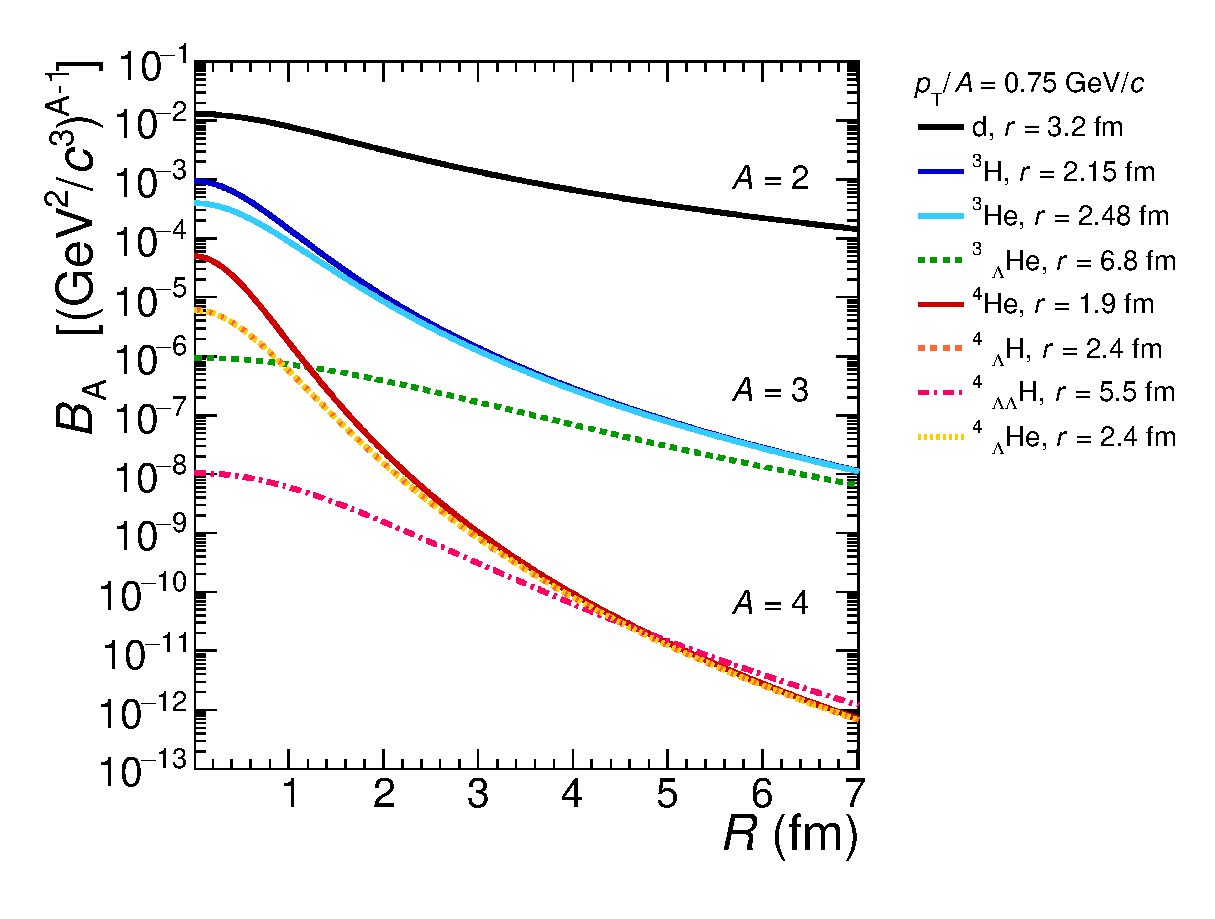
\includegraphics[width=0.8\textwidth]{coalescenceBA075.eps}
\caption{(Color online) Coalescence parameter $B_A$ as a function of the source radius $R$ as predicted from the coalescence model (Eq.~\ref{eq:master}) for various composite objects with \pt$/A$~=~0.75~\GeVc. For each (hyper-)nucleus, the radius $r$ used for the calculation is reported in the legend.}
\label{Fig:BA}
\end{center}
\end{figure} 

\section{Comparison with data}

\begin{figure}[htb]
\begin{center}
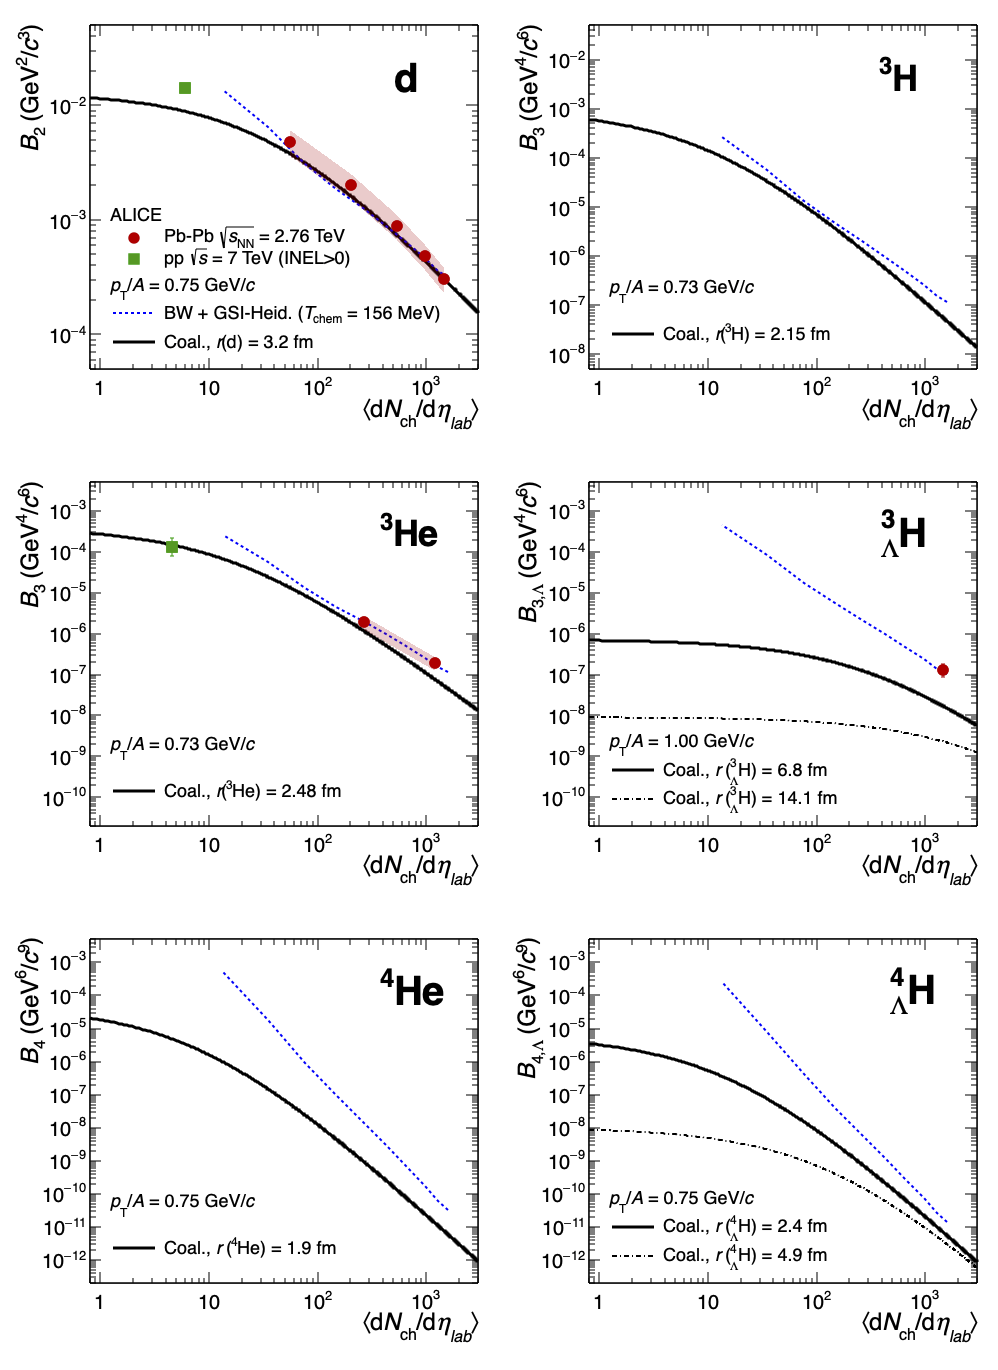
\includegraphics[width=\textwidth]{coal2Thermal2alice.png}
\caption{(Color online) Coalescence parameter $B_A$ as a function of the average charged particle multiplicity density for various (hyper-)nuclei, up to $A = 4$. The coalescence calculations (continuous or dashed-dotted black lines) are compared to the thermal+blast-wave predictions (dashed blue line), as well as to pp (green square) and \PbPb~(red circles) collision data from ALICE~\cite{ALICE:nucleipp2017,ALICE:deuteronppPbPb2015,Adam:2015yta}. }
\label{Fig:comparison}
\end{center}
\end{figure} 

\begin{figure}[htb]
\begin{center}
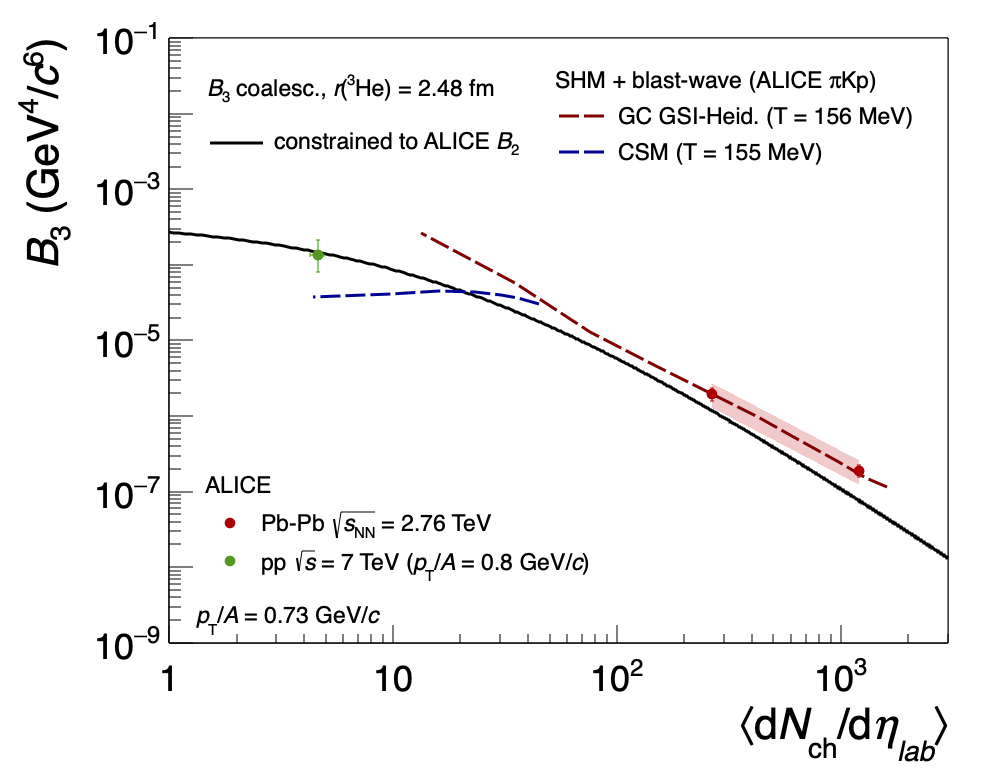
\includegraphics[width=0.8\textwidth]{B3vsMult073.png}
\caption{(Color online) Coalescence parameter $B_3$ for \hethree~as a function of the average charged particle multiplicity density. The coalescence calculation (continuous black line) is compared to two thermal+blast-wave predictions (dashed lines), obtained by using the Grand Canonical (GC, red)~\cite{Andronic:2017} and Canonical Statistical Model (CSM, blue) \cite{Vovchenko:2018fiy} expectations for the \hethree~yield, respectively. ALICE data from pp (green circles) and \PbPb~(red circles) collisions~\cite{ALICE:nucleipp2017,ALICE:deuteronppPbPb2015} are reported. }
\label{Fig:3He}
\end{center}
\end{figure} 

\newpage
\bibliographystyle{utphysnt} 	
\bibliography{biblio}
\end{document}

